\section{Introduction}

We naturally categorize items we encounter daily for ease of storage, processing, and decision-making. For example we know instinctively that regardless of shape and form, all lamps form a 'lamp' category based on its function. Several factors determine how we categorize items. Depending on the complexity of rules that determine categories, some categorizations are easier than others \cite{shepard1961learning, nosofsky1994comparing}. Category variability can modulate how often exemplars are classified into that categories \cite{cohen2001category}.

The order of presentation items in category learning tasks has been shown to be an important factor in how category diagnostic features are learned. In particular, when items are presented in a blocked categorical design, participants seem to learn the similarities between the same category items. On the other hand, when items are presented as an interleaved design, participants seem to focus more on learning the features that differentiate the underlying categories \cite{carvalho2017sequence}. As a result of order-dependent differing focus on category diagnostic features, interleaved presentations seem to benefit general category learning. In most prior category-learning tasks assessing order of presentation effects, participants are explicitly asked to learn the underlying categories. There appear to be clear differences when participants focus on learning categories based on how exemplars of these categories are presented \cite{kornell2008learning, kornell2010spacing, whitehead2021transfer, vlach2008spacing, carvalho2014putting, carvalho2017sequence}. In this article, we investigate the effects of order of presentation when category learning is implicit. 

One primary focus on category learning through order of presentation is comparing blocked or interleaved exemplar presentations. For example, \cite{kornell2008learning} showed participants paintings made by two different painters. The order of presentation during exposure was modulated to either be blocked (paintings of one artist shown together followed by the second artist) or interleaved (paintings made by both artists were mixed). When presented with new paintings, and asked which of the two studied artists made them, participants who were exposed to the interleaved format were found to be more accurate at guessing the creator. Category learning also improved for interleaved presentation compared to blocked presentation when tested on items where relevant category features were visually occluded \cite{whitehead2021transfer}. When three-year-old children are tested on the generalization of category-specific features, they appear to benefit from the spaced study of exemplars as compared to a blocked \cite{vlach2008spacing}. By modulating the similarity of presented items, interleaved presentation was found to be better than blocked presentation design on generalization performance particularly when learned exemplars were more visual \cite{kornell2008learning, carvalho2014putting}. 

Interleaved presentation has been theorized to improve in category induction because of context-based variability during encoding \cite{glenberg1979component}. Particularly, for each presented item, an observer will store both the item-specific features along with the context in which the item is encoded. During interleaved presentation, a category diagnostic feature gets encoded under different contexts. Thus, that diagnostic feature will be recalled when tested on novel category items within that context. 

Two theories have been proposed to explain this discriminability-based advantage of interleaving. According to the attention attenuation account, when categories are blocked, participants may think that they have learned the relevant category features after viewing a few items and stop paying attention to additional exemplars of the \cite{kornell2010spacing}. On the other hand, according to the discrimination account, the interleaved presentation allows participants to directly compare the differences between exemplars of different categories that are presented close to each other thereby highlighting these differences \cite{kornell2008learning}. In a direct test \cite{wahlheim2011spacing} found that when participants were shown pairs of exemplars, each belonging to a different category, the interleaving benefit was magnified compared to when they were presented as single items. The authors posit that showing pairs of exemplars would enable participants to carefully study and infer distinctions between category features and hence improve categorization performance .Furthermore, the authors find evidence against the attention attenuation theory by observing that classification performance did not differ as a function of the position in which the exemplar was presented in a stream.

This benefit of interleaved presentation is shown to be modulated by the `level' at which categorization occurs. For example, when \cite{mack2015dynamics} modulated exposure time to individual exemplars along with order of exposure, they found that interleaved presentation was no longer beneficial under short exposure conditions particularly when participants were asked to make a more abstract, `super-ordinate level categorization. On the other hand, when exemplars were presented in a blocked format, a lower, `basic' level categorization was hindered. Thus, category knowledge through order of presentation can be modulated by the level of categorization participants are asked to produce.

It is clear that order of presentation of categories matters during explicit category learning. However, the effect of such order of presentation has not been investigated when category learning is implicit. Indeed recent work shows that participants do acquire category knowledge that when presented implicitly instead of being explicitly asked to learn categories. \cite{unger2022ready} found that assessed on category knowledge, participants appeared to learn category structures without being explicitly instructed to do so. This category knowledge was modulated by the strength of association of the category diagnostic features. \cite{unger2023without} later found that when presented with implicit feature-based categories during a cover task, participants were sensitive towards category diagnostic knowledge. 

More evidence for incidental category learning comes from auditory cognition. \cite{gabay2015incidental} found that participants were sensitive to audio categories learned implicitly as measured by increased reaction times when audio-category-to-response mapping was altered. Incidental category knowledge is further modulated by the sampling category distributions from which exemplars are drawn. \cite{roark2018task} show that probabilistic sampling of exemplars leads to weaker category learning compared to deterministic sampling. Incidental category learning can be further enhanced by task-relevant and disrupted by task-irrelevant feature-to-category mappings \cite{roark2022representational}. Incidental learning may also be disadvantaged compared to supervised intentional learning when categories are non-linearly separable \cite{love2002comparing}.

More incidental category learning has been studied under the `unsupervised' category learning. Participants could infer rules based on correlating features without being explicitly asked to categorize during exposure \cite{billman1996unsupervised}. Category-related items were recognized better when presented close to each other then when category-unrelated items were \cite{medin1994presentation} with people being able to sort stimuli by a single dimension\cite{medin1987family}. Models of categorization have attempted to explore mechanisms of such unsupervised category learning.  SUSTAIN \cite{love2004sustain} seems to explain several of these unsupervised category learning phenomena using a distributed representation whereas ALCOVE \cite{kruschke2020alcove} further provides for error based diagnostic feature attention learning in GCM \cite{nosofsky2011generalized, nosofsky1986attention}.

While implicit category learning appears to be consistent and dependent on several aspects of the underlying categories, unlike explicit category learning, it is unclear whether implicit category learning enjoys the same advantage when category exemplars are presented in an interleaved vs. a blocked design. Most implicit categorization tasks involve manipulation of features as opposed to manipulation of the temporal order of exposure. 

\subsection{Simulating temporal advantage}

Prior work in implicit event boundaries has shown that stimuli shown closer to each other in time develop similar representations in memory and in particular the hippocampus and the medial temporal lobe \cite{schapiro2013neural, turk2019hippocampus, bonner2021object}. Context representations through, for example, SR, can provide algorithmic accounts for such increased similarity between co-occurring events. For example, consider events occurring as the graph in figure \ref{fig:category-graph-structures}

\begin{figure}[ht]
    \centering
    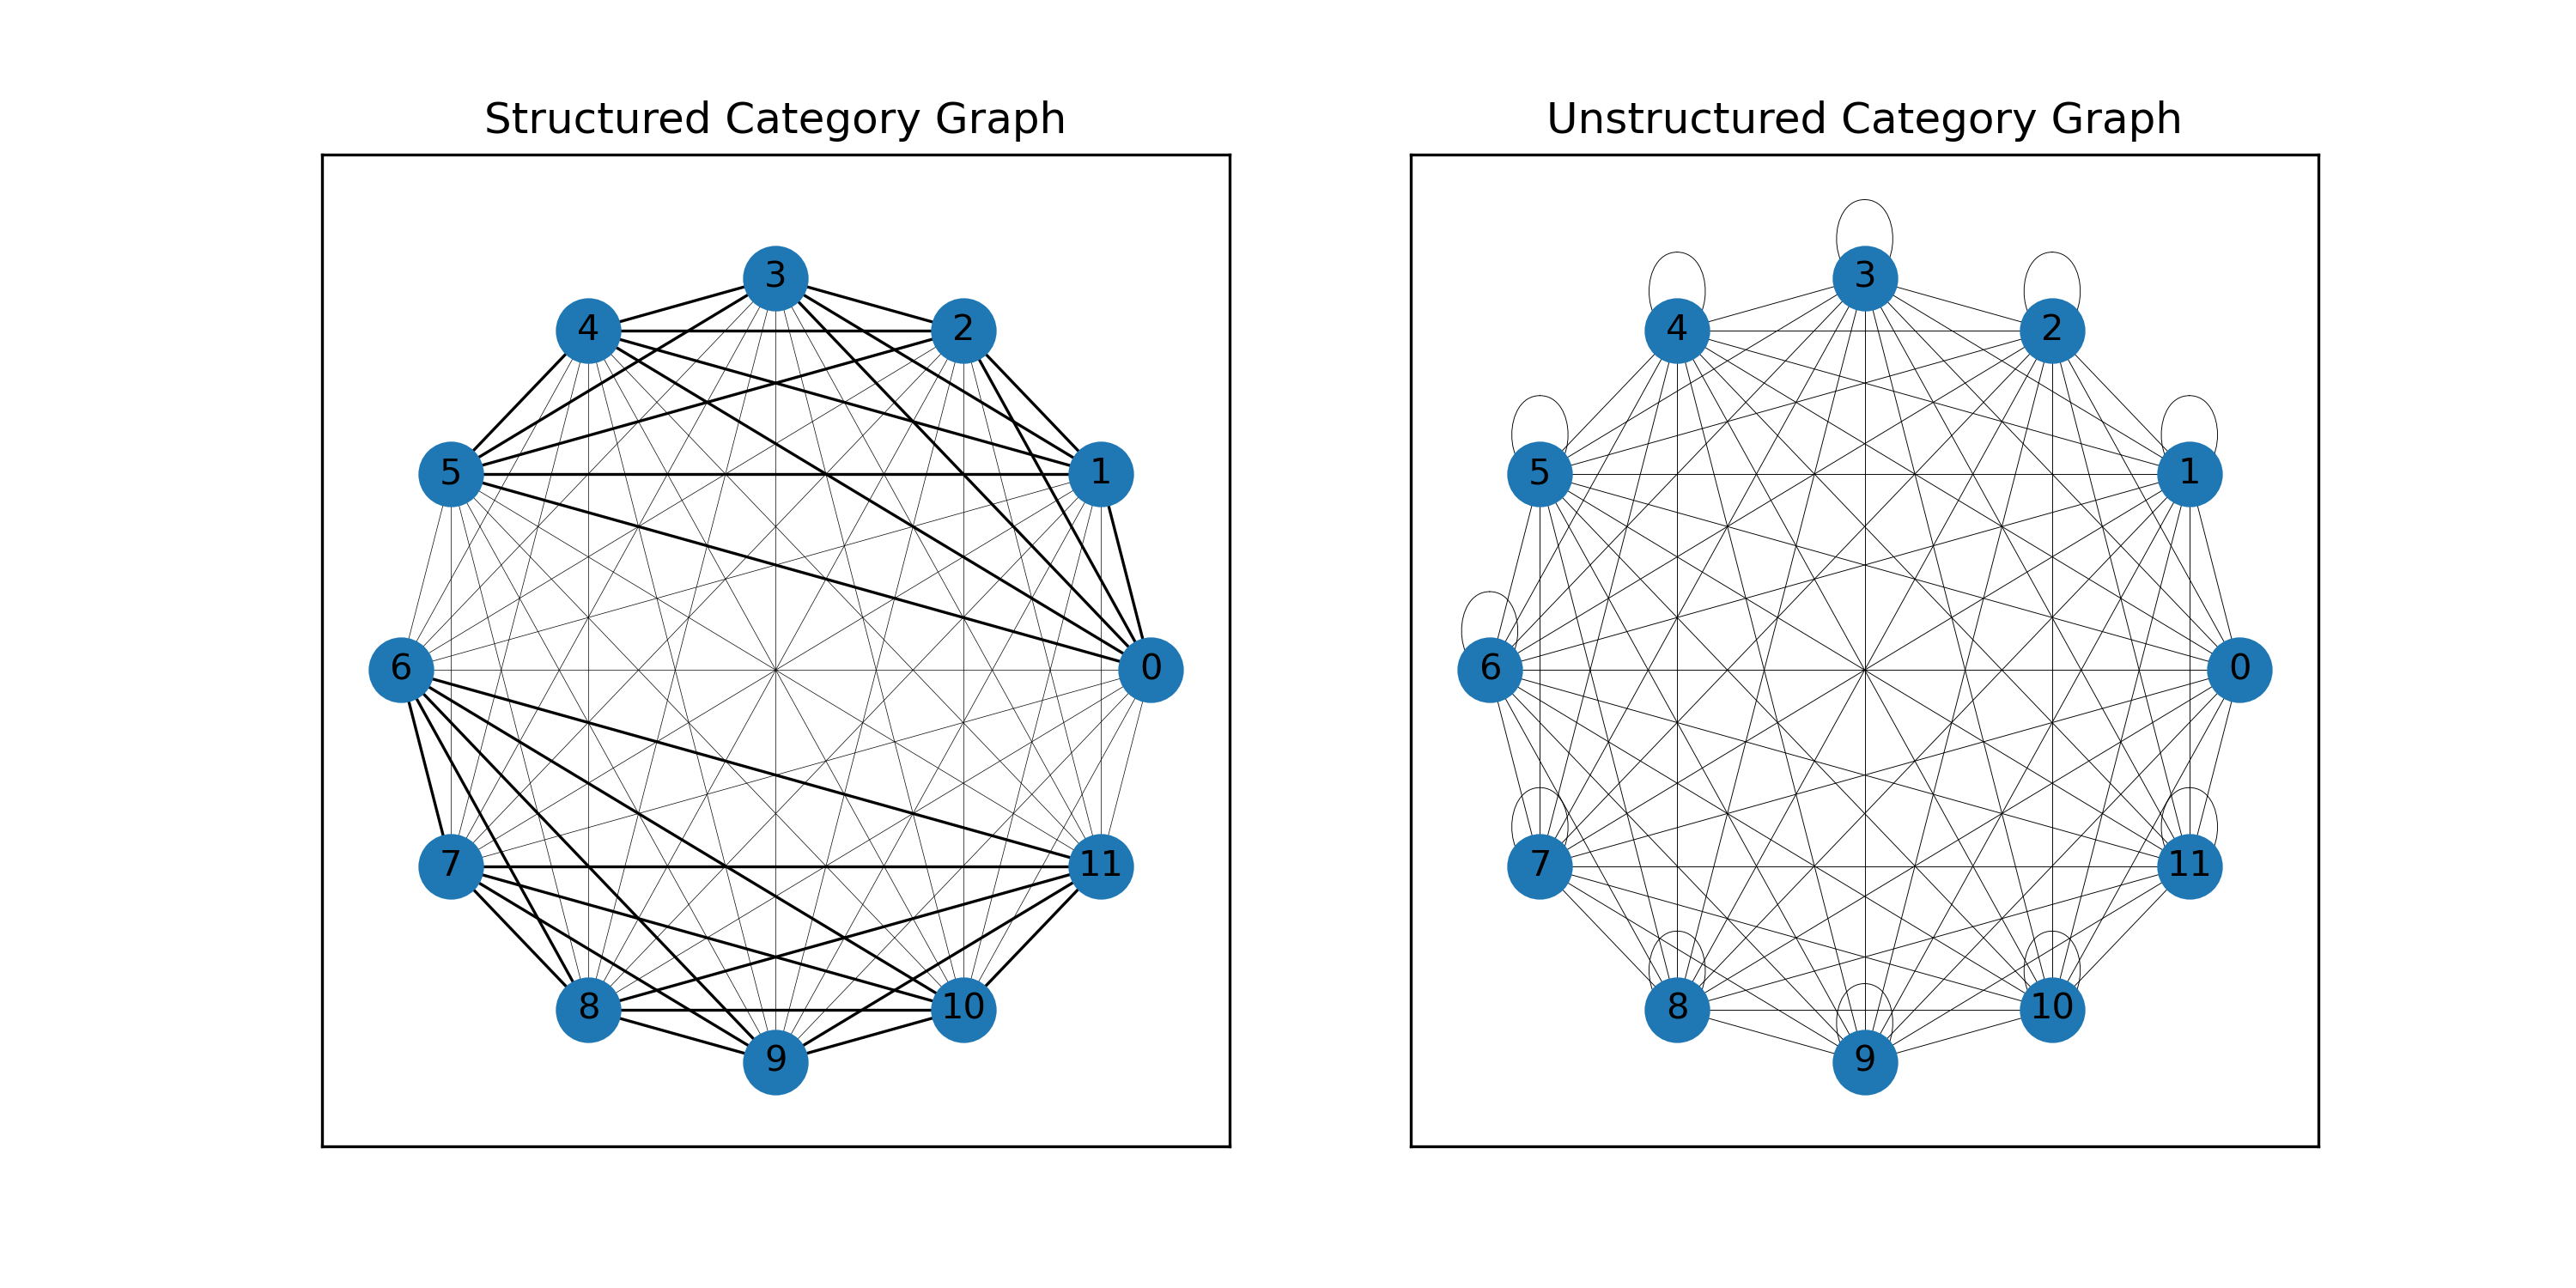
\includegraphics[width = \textwidth]{chapter_notebooks/chapter_4/figures/cat_graphs.png}
    \caption{Graph structures used in categorization experiments. Edge thickness indicates transition probabilities between nodes.}
    \label{fig:category-graph-structures}
\end{figure}

All nodes in both graphs are connected to all other nodes. However, connectivity in the graph on the left is determined by weighted edges -- darker edges are 4 times as likely to be traversed as lighter edges. On the other hand, all edges (including within-node edges) are equivalent in the graph on the right. Since SR represents expected transition probabilities between each pairs of nodes, a (weighted) random walk through such a graph structure produces distinctive representations of context (Figure \ref{fig:category-sr-sims}).

\begin{figure}
    \centering
    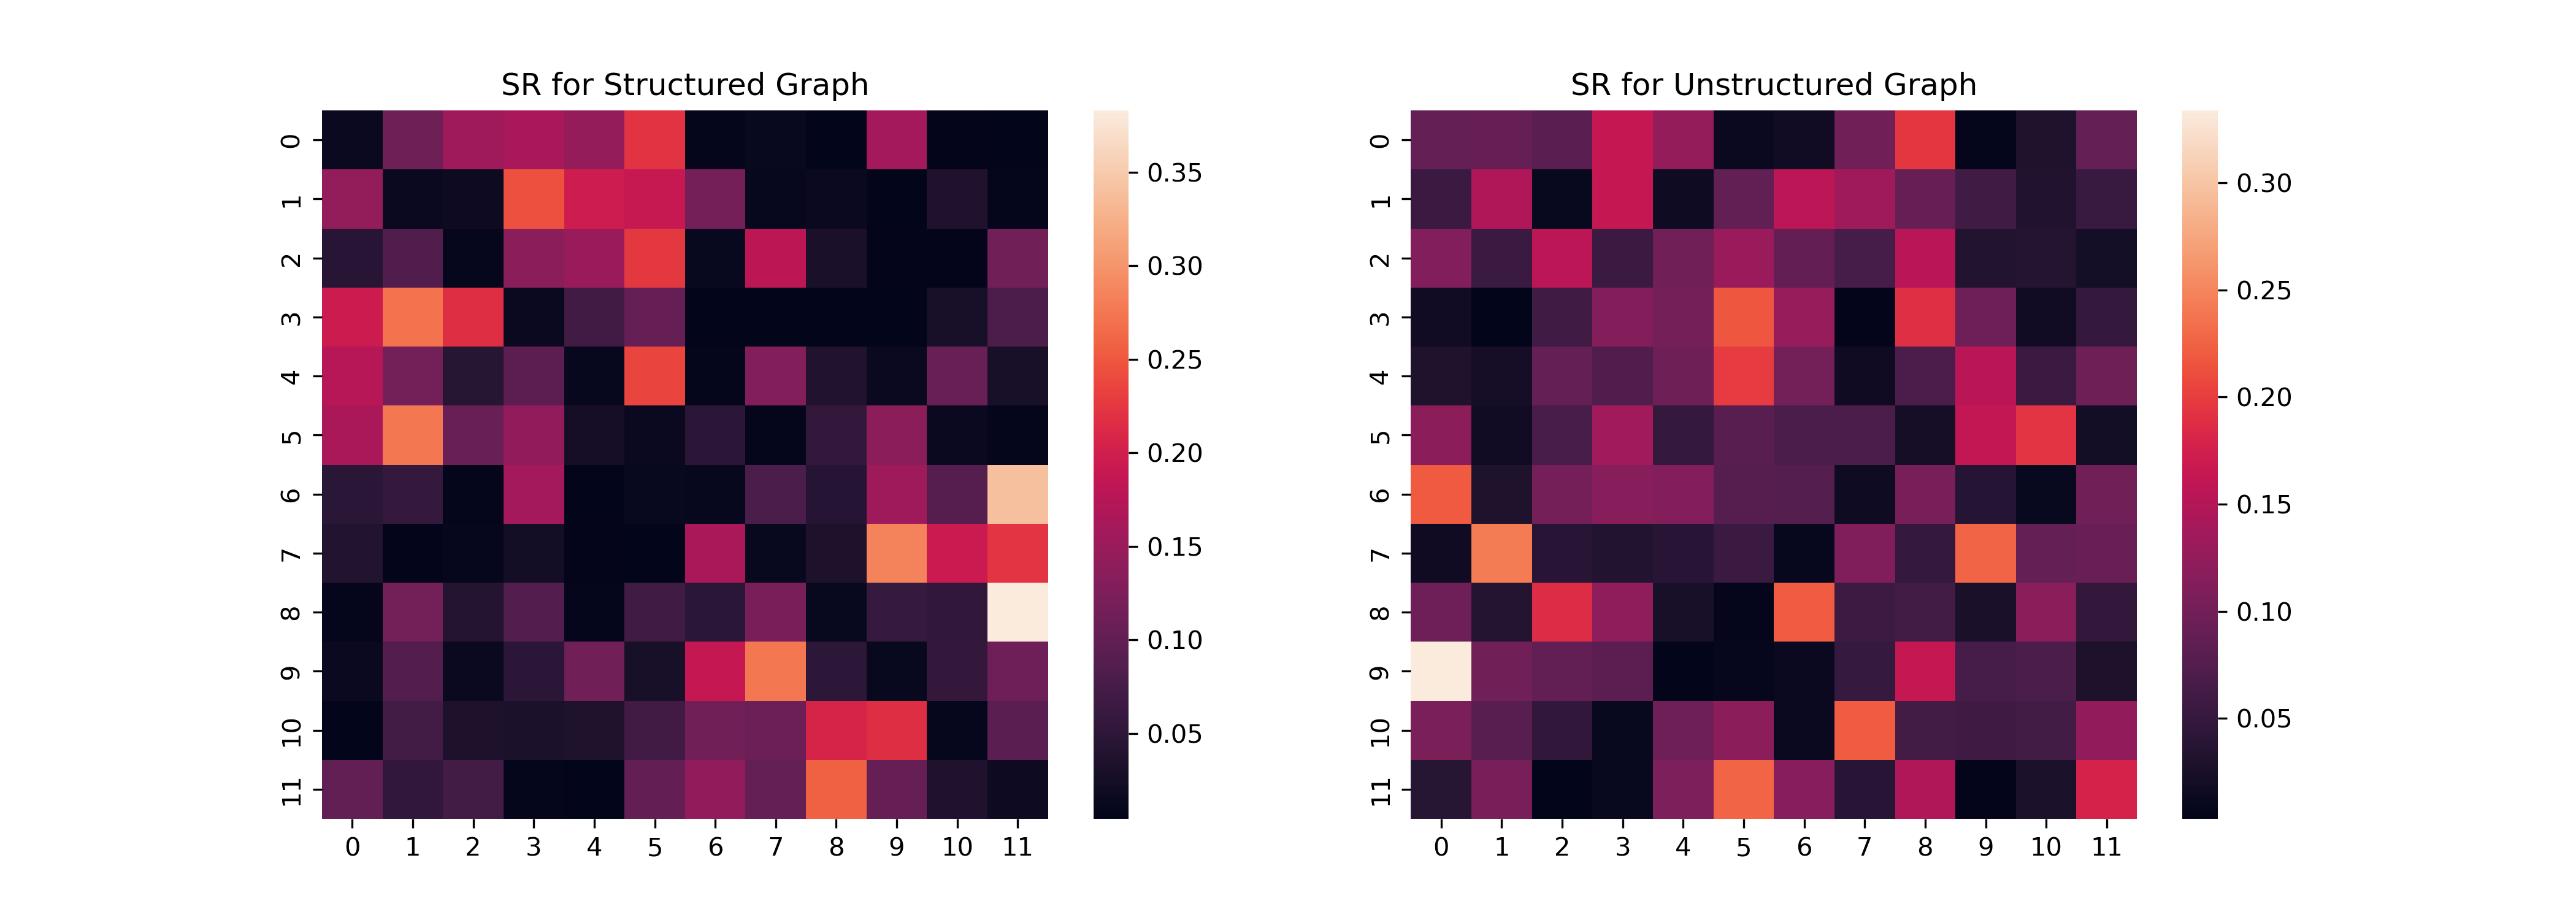
\includegraphics[width = \textwidth]{chapter_notebooks/chapter_4/figures/category-sr-sims.png}
    \caption{SR representations of graph structures used for categorization.}
    \label{fig:category-sr-sims}
\end{figure}

The SR representations thus provides a natural way of representing two temporally defined categories. The key question I ask in this chapter is whether temporal proximity can lead to an increased realization of an inherent visual category structure. That is, in tasks where participants are are unaware of categorization tests or of category diagnosticity of some visual features, does temporal proximity of same-category items lead to a realization of category-diagnosticity of features?

To simulate temporal advantage, I follow the exemplar matching principles from GCM \cite{nosofsky1994comparing,rouder2004comparing,nosofsky2011generalized,nosofsky1986attention}. However, unlike the standard GCM which is used to model categorization learned through explicit feedback of category membership, the tasks presented later in this chapter will not provide any information or an explicit learning signal regarding the true category membership. Additionally, the categorization tests in experiments of this chapter will \textit{not} compare new exemplars with stored category exemplars in memory (especially since no stored exemplars will have an explicit category label). Instead, participants will be asked to compared \textit{studied} exemplars with two new exemplars which maintain most features of the studied exemplars while varying either on a subset of category diagnostic features or category non-diagnostic features. The goal is to thus investigate whether temporal co-occurences cause participants to notice features that are category diagnostic. Finally, unlike traditional GCM, tasks in these experiments use binary valued features to allow for better control of the number of possible feature values and feature dimensions. Few modifications to the formulation of the GCM were therefore necessary. This modified GCM can be formally described as follows:

\begin{equation}
    \begin{aligned}
        d_{ij} = \sum_{m} w_m x_{im} \oplus x_{jm} \\
        s_{ij} = exp(-d_{ij}) \\ 
        p(i|c) = \frac{s_{ic}}{s_{ic} + s_{jc}} 
    \end{aligned}
\end{equation}

where $d_{ij}$ is the bitwise XOR distance between two binary feature vectors representing items $i$ and $j$. $w_m$ is the weighte associated with each of the features. $s_{ij}$ is the similarity between items $i$ and $j$. $p(i|c)$ represents the probability of selecting option $i$ between options $i$ and $j$ given similarities of item $c$ with items $i$ and $j$. Notably, in this formulation of the GCM, the weights of dimensions are only relevant upon mismatch between those features (an assumption in line with other recognition memory and categorization theories such as the Diagnostic Feature Detection Theory \cite{wixted2014signal}).

To incorporate the role of SR-driven context representation, I further assume that the attention weights $w_m$ towards each feature are modulated by SR activations. Specifically, when a stimulus transition is experienced, features that stay constant are facilitated with an increased importance. The magnitude of this increase is assumed to be proportional to the SR representation of the two items. Formally, 

\begin{equation}
    \begin{aligned}
        w_m = \sum_{i, j}^{i_m = j_m} M(i, j)
    \end{aligned}
\end{equation}

Where $M(i, j)$ is the SR activation of item $j$ in item $i$. Feature attentions weights, thus develop over time as items co-occur and the SR matrix $M$ consolidates to represent two clusters seen in figure \ref{fig:category-sr-sims}. This formulation allows to simulate an upper bound of category membership (for a given number of trials and set of parameters). Figure \ref{fig:sr-cat-selection-sims} shows this upper bound for the structured graph where transitions are differentially weighted to create temporal clusters relative to the unstructured graph where all transitions are equally likely. 

\begin{figure}[ht]
    \centering
    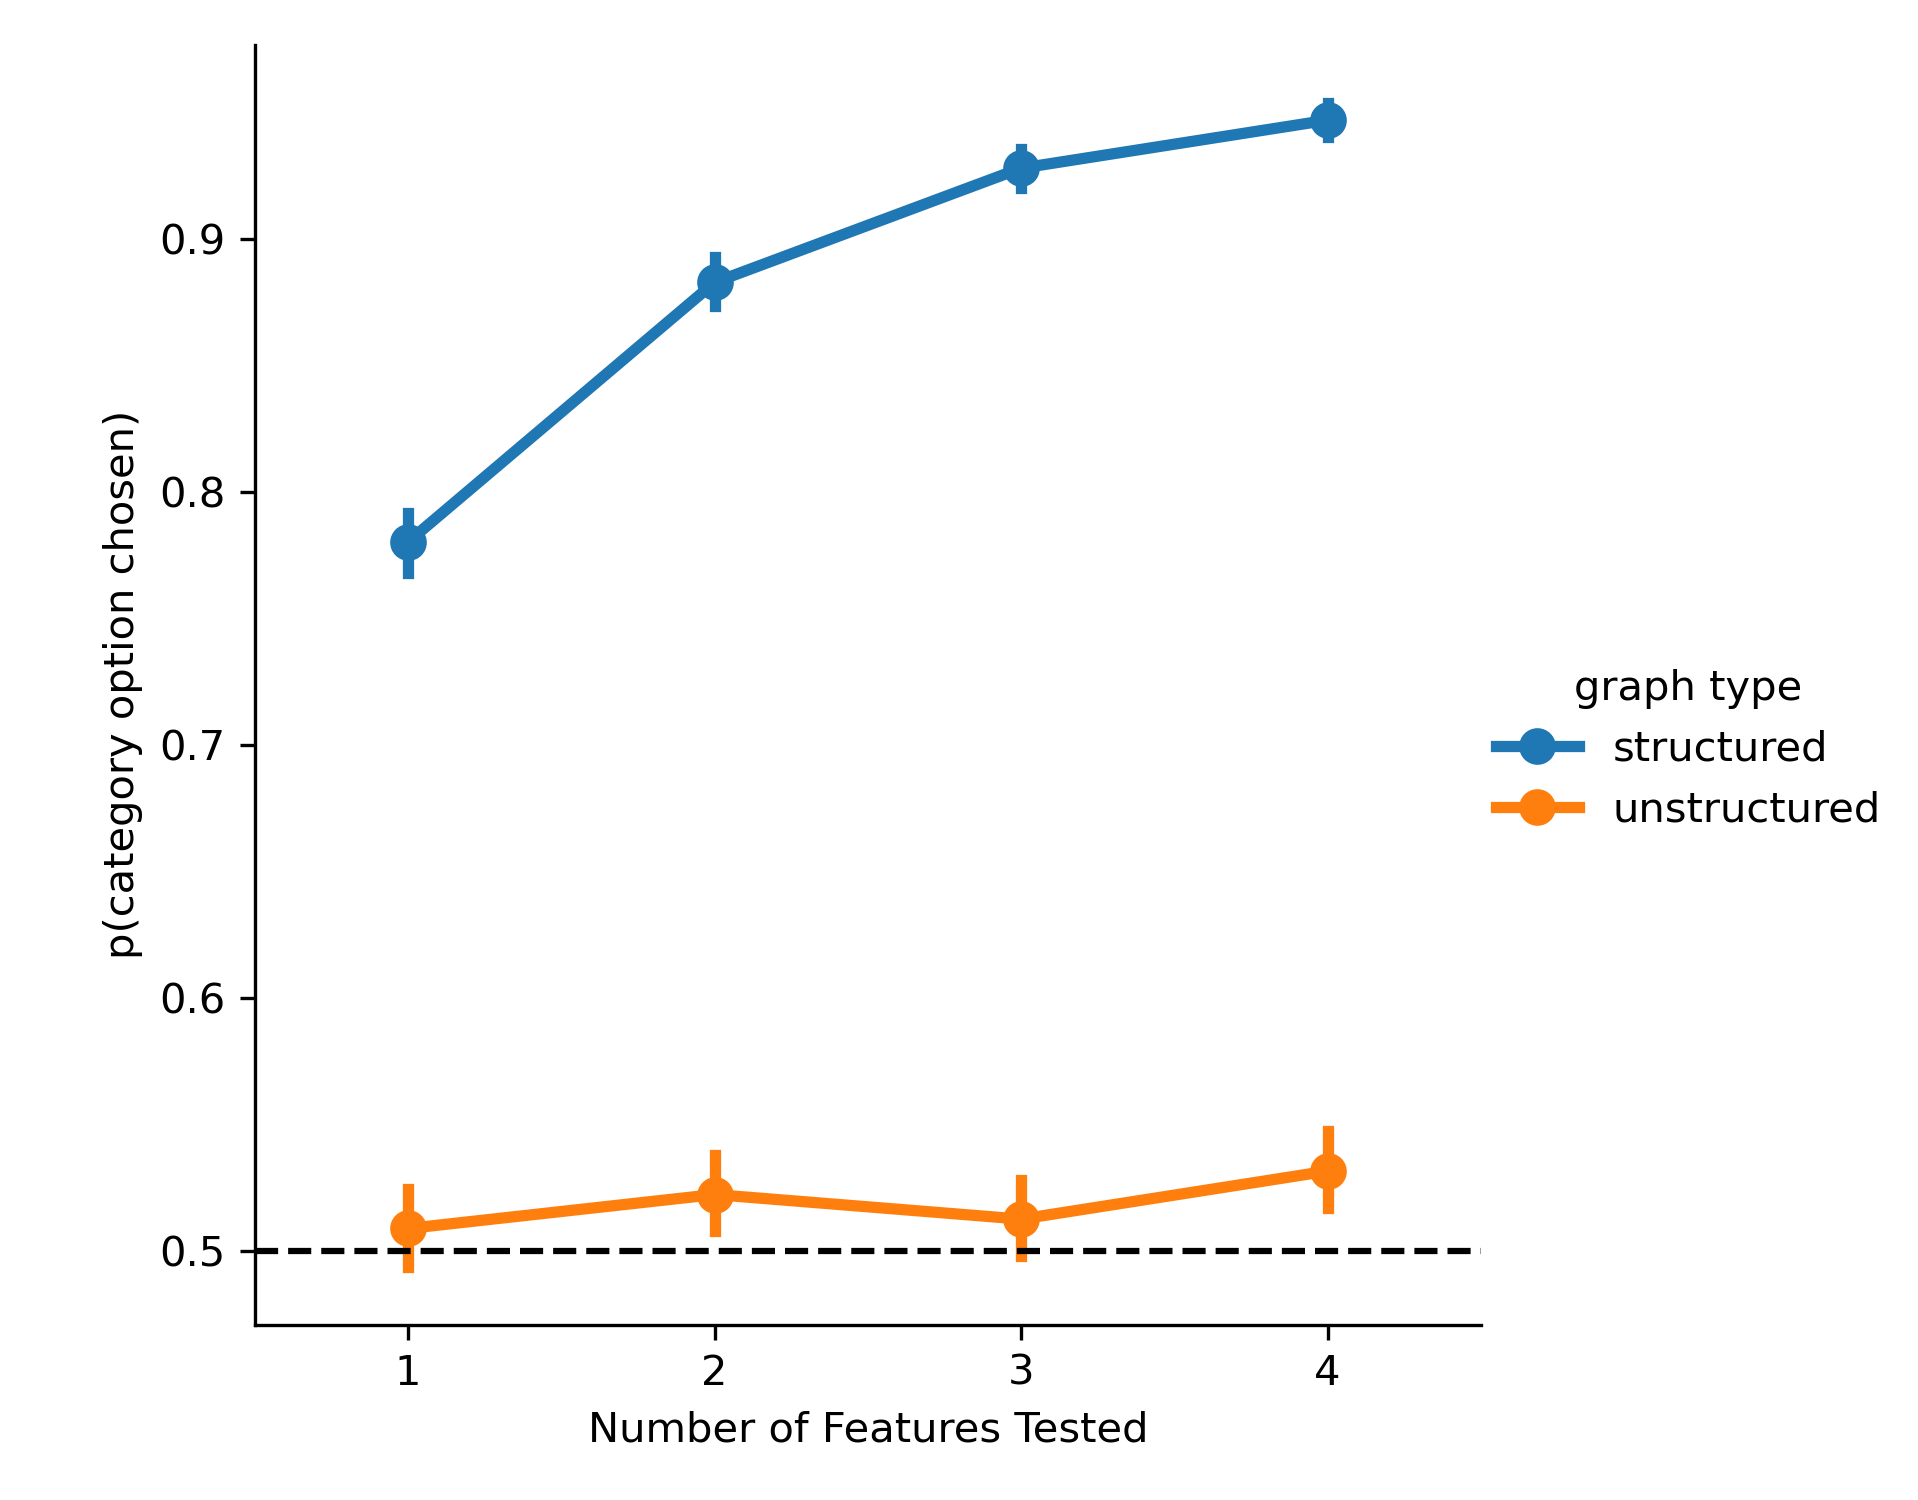
\includegraphics[width = \textwidth]{chapter_notebooks/chapter_4/figures/cat_simulations.png}
    \caption{Simulated proportions of test trials where the option selected will be consistent on its category diagnostic features assuming feature weights modulated by SR.}
    \label{fig:sr-cat-selection-sims}
\end{figure}

In the experiment presented next, I aim to test this model prediction. In particular, participants who are explored to structured graph in binary featured stimuli will consolidate their experience and categorize items based on their (temporally defined) category diagnostic features. Here category diagnostic features are defined by consistency in the values of a feature among aliens that are presented closer to each other. That is, if the probability of going from an alien associated with node 0 to an alien associated to node 1 is high, common features between these aliens are labeled as category diagnostic whereas the features that stay consistent during low probability transitions are labeled as category non-diagnostic features. 

\section{Experiment 3a}

\subsection{Methods}

\subsubsection*{Participants}
58 participants were recruited online via prolific to participate in the study designed in Psychopy \cite{peirce2007psychopy}. Participants were paid \$5 for their time. All study procedures were approved by the University of Massachusetts Institutional Review Board. 

\subsubsection*{Stimuli creation and assignment}
Alien stimuli for used in this study were created using python's Matplotlib library \cite{hunter2007matplotlib}. Each alien consisted of 8 binary valued features, evenly distributed across 4 dimensions (shape, size, color, and orientation). The 8 binary valued features comprised of head color (brown or orange) and torso color (green or purple) for the color dimension; eyes (large or small circles) and arms (large or small lengths) for the size dimension; nose (square or circle) and bellybutton (square or circle) for the shape dimension, and antenna (pointing inwards or outwards) and feet (pointing inwards or outwords) for the orientation dimension. 

One randomly chosen feature from each dimension was chosen as a `category diagnostic' feature whereas the other was deemed as non-diagnostic. Category diagnosticity of a feature was determined based on cluster assignment in figure \ref{fig:category-graph-structures}. Specifically, all category diagnostic features in the same cluster were assigned the same value (for example, all green torsos). In order to equate the number of features of the non-category diagnostic feature, three stimuli in a cluster were assigned the same value of a non-category diagnostic features whereas the other three were assigned a different value (e.g. three orange heads and three brown heads). The table below shows example feature values for the categorization experiment. 

\begin{table}
\centering
\label{tab:category-features-example}
\caption{An example set of stimuli with Antenna Orientation, Eye size, Head Color and Nose shape are category diagnostic based on proximity of occurrence.}
\begin{tabular}{lrrrrrrrr}
    \toprule
    Feature Elements & Antenna & Arms & Bellybutton & Eyes & Feet & Head & Nose & Torso \\
    Stimulus &  &  &  &  &  &  &  &  \\
    \midrule
    1 & 0 & 1 & 0 & 0 & 1 & 0 & 0 & 0 \\
    2 & 0 & 0 & 1 & 0 & 0 & 0 & 0 & 1 \\
    3 & 0 & 0 & 0 & 0 & 1 & 0 & 0 & 1 \\
    4 & 0 & 1 & 1 & 0 & 0 & 0 & 0 & 0 \\
    5 & 0 & 1 & 0 & 0 & 0 & 0 & 0 & 1 \\
    6 & 0 & 0 & 1 & 0 & 1 & 0 & 0 & 0 \\
    7 & 1 & 1 & 0 & 1 & 1 & 1 & 1 & 0 \\
    8 & 1 & 0 & 1 & 1 & 0 & 1 & 1 & 1 \\
    9 & 1 & 0 & 0 & 1 & 1 & 1 & 1 & 1 \\
    10 & 1 & 1 & 1 & 1 & 0 & 1 & 1 & 0 \\
    11 & 1 & 1 & 0 & 1 & 0 & 1 & 1 & 1 \\
    12 & 1 & 0 & 1 & 1 & 1 & 1 & 1 & 0 \\
    \bottomrule
\end{tabular}

\end{table}

This formulation allows to thus test whether temporal proximity of consistent features leads to an increased weights on features that co-occur or whether temporal proximity of the \textit{change} in features (i.e. the non-diagnostic features) leads to increased weights in those features. 

        
\subsubsection*{Design and Procedure}

The experiment consisted of two phases; an exposure phase and a categorization phase. During the exposure phase, participants were shown one of 12 aliens at a time. After a brief period the alien flipped (randomly) left or right. Participants were asked to hit a key to indicate which direction the alien flipped. 

The order of stimulus presentation was controlled by a weighted random walk through the graph structure in figure \ref{fig:category-graph-structures}. 29 participants were presented a stimulus stream following the weighted structured graph (left panel) whereas the other 28 were presented a stimulus stream following the unstructured graph (right panel). For participants experiencing structured weighted random walk, category diagnostic features remained consistent across transitions with 80\% probability and changed with a 20\% probability whereas the category non-diagnostic features changed with an 80\% probability and remained constant with 20\% probability. On the other hand, the participants in unstructured exposure condition experienced an equal probability of change across all features. 

\begin{figure}
    \centering
    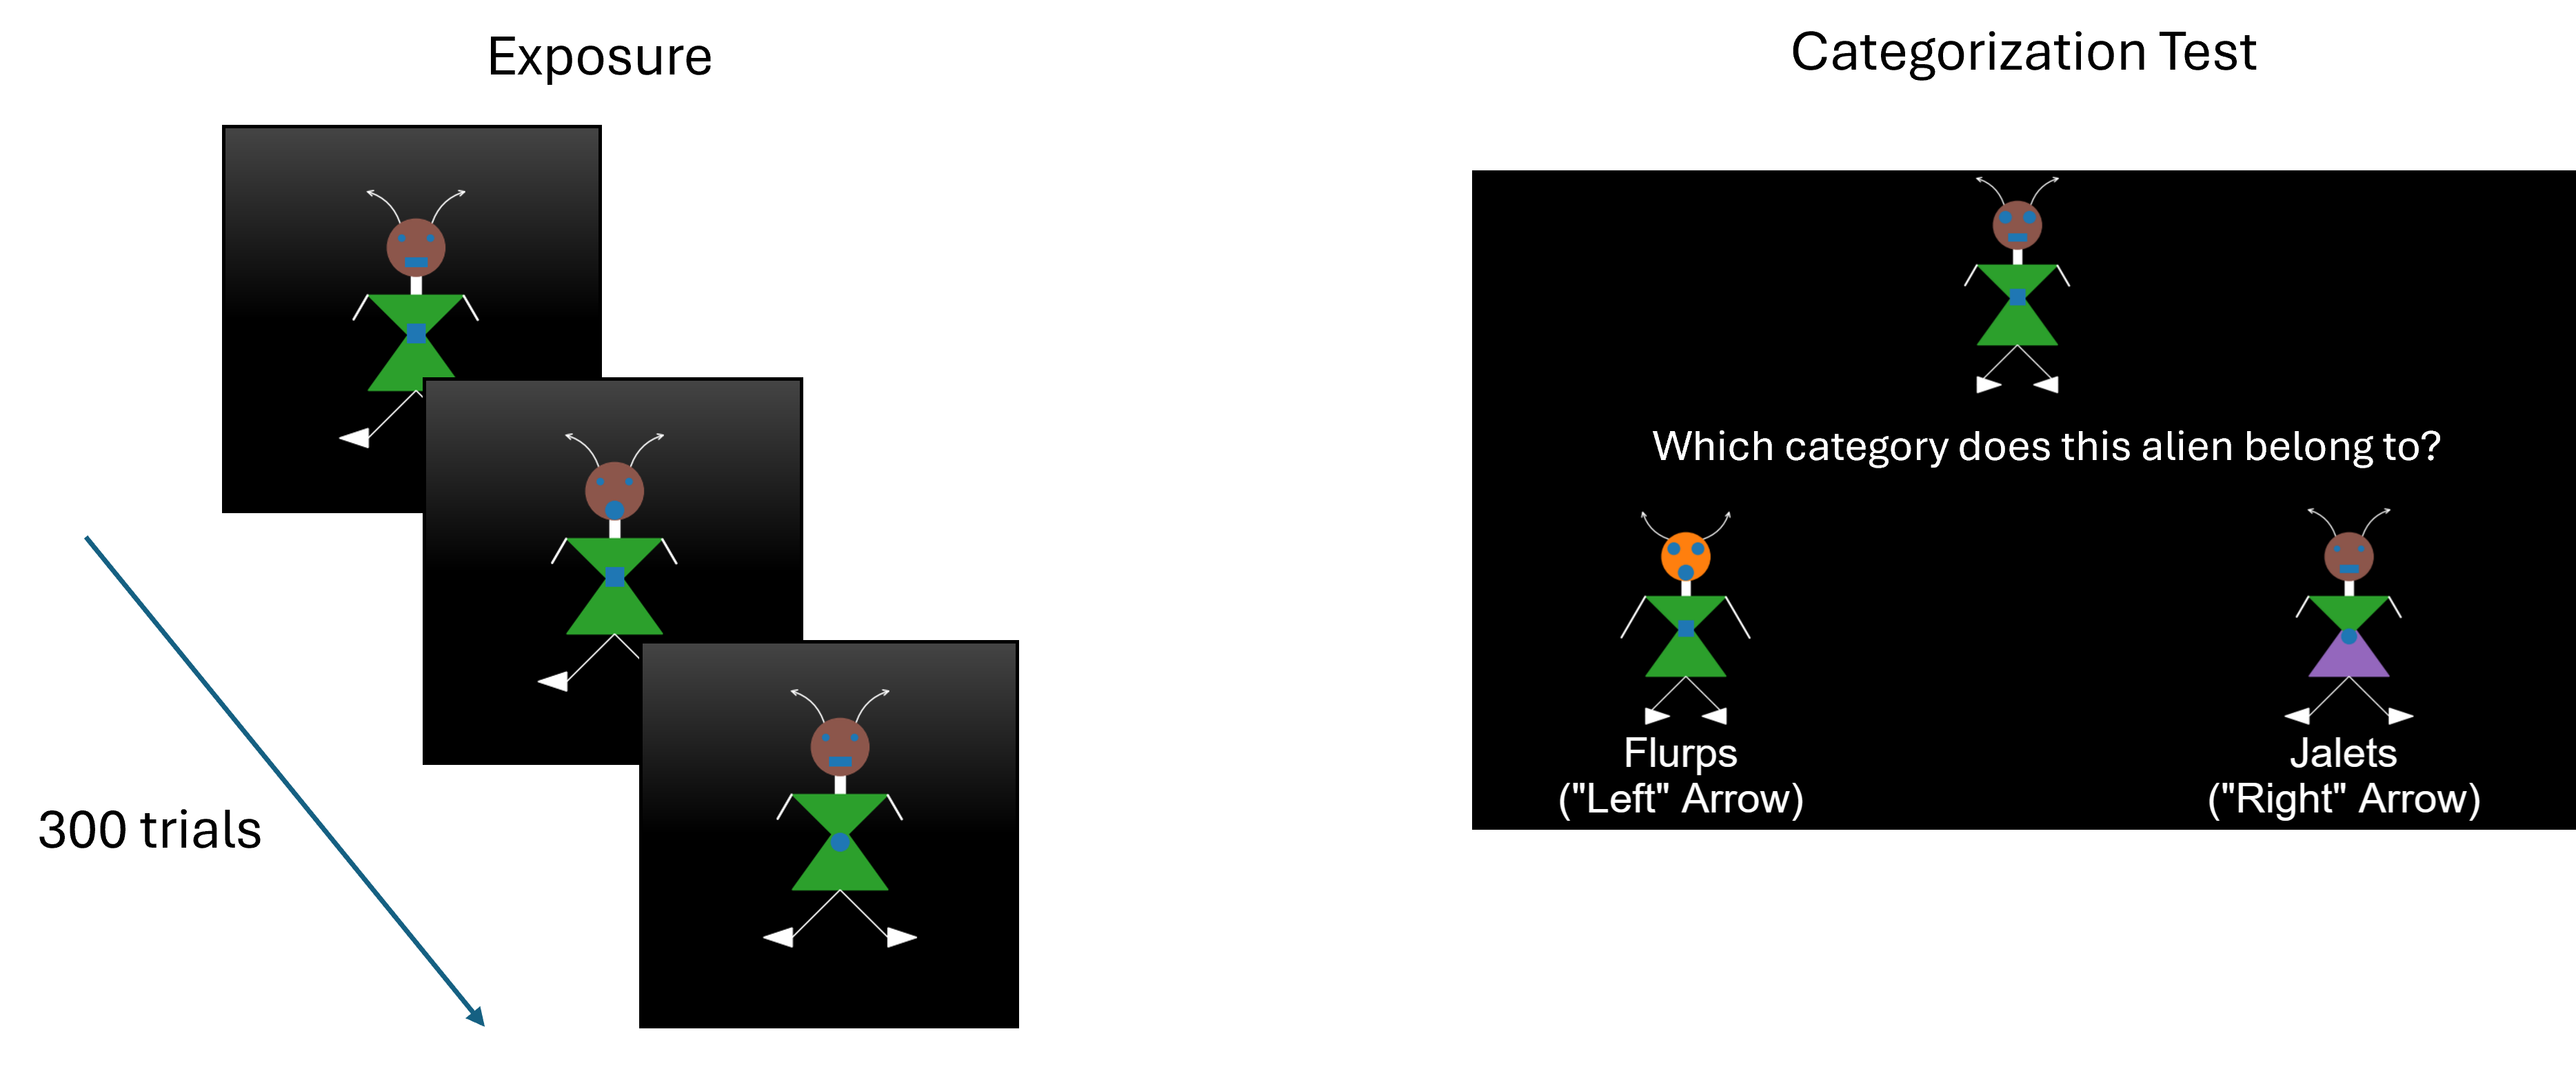
\includegraphics[width = \textwidth]{chapter_notebooks/chapter_4/figures/exp45_design.png}
    \caption{Experiment design schematic for experiments 4a and 4b.}
    \label{fig:exp45-deisgn}
\end{figure}

The general experiment design is shown in figure \ref{fig:exp45-deisgn}. After 300 trials of exposure, participants were asked to categorize the aliens they had seen at exposure. Specifically, for each of the 12 aliens, two options were provided. The category option matched on all category diagnostic features and all but $n$ category non-diagnostic features (where $n in [1,4]$) and the non-category option matched on all category non diagnostic features and all but $n$ category diagnostic features. Participants were asked to select which of the two option does the studied exemplar more relate to in their visual properties. Thus, if a participant selected the category option more often in the structured case, temporal proximity of consistent features increases the weight of shared feature values. On the other hand, if a participant selected the non-category option more often in the structured case, temporal proximity of non-consistent features increases weights of the non-shared feature values.

\subsection{Results}

\begin{figure}[h]
    \centering
    \caption{Proportion of categorization trials where a category diagnostic feature (one which remained more consistent over time) was used to categorize items.}
    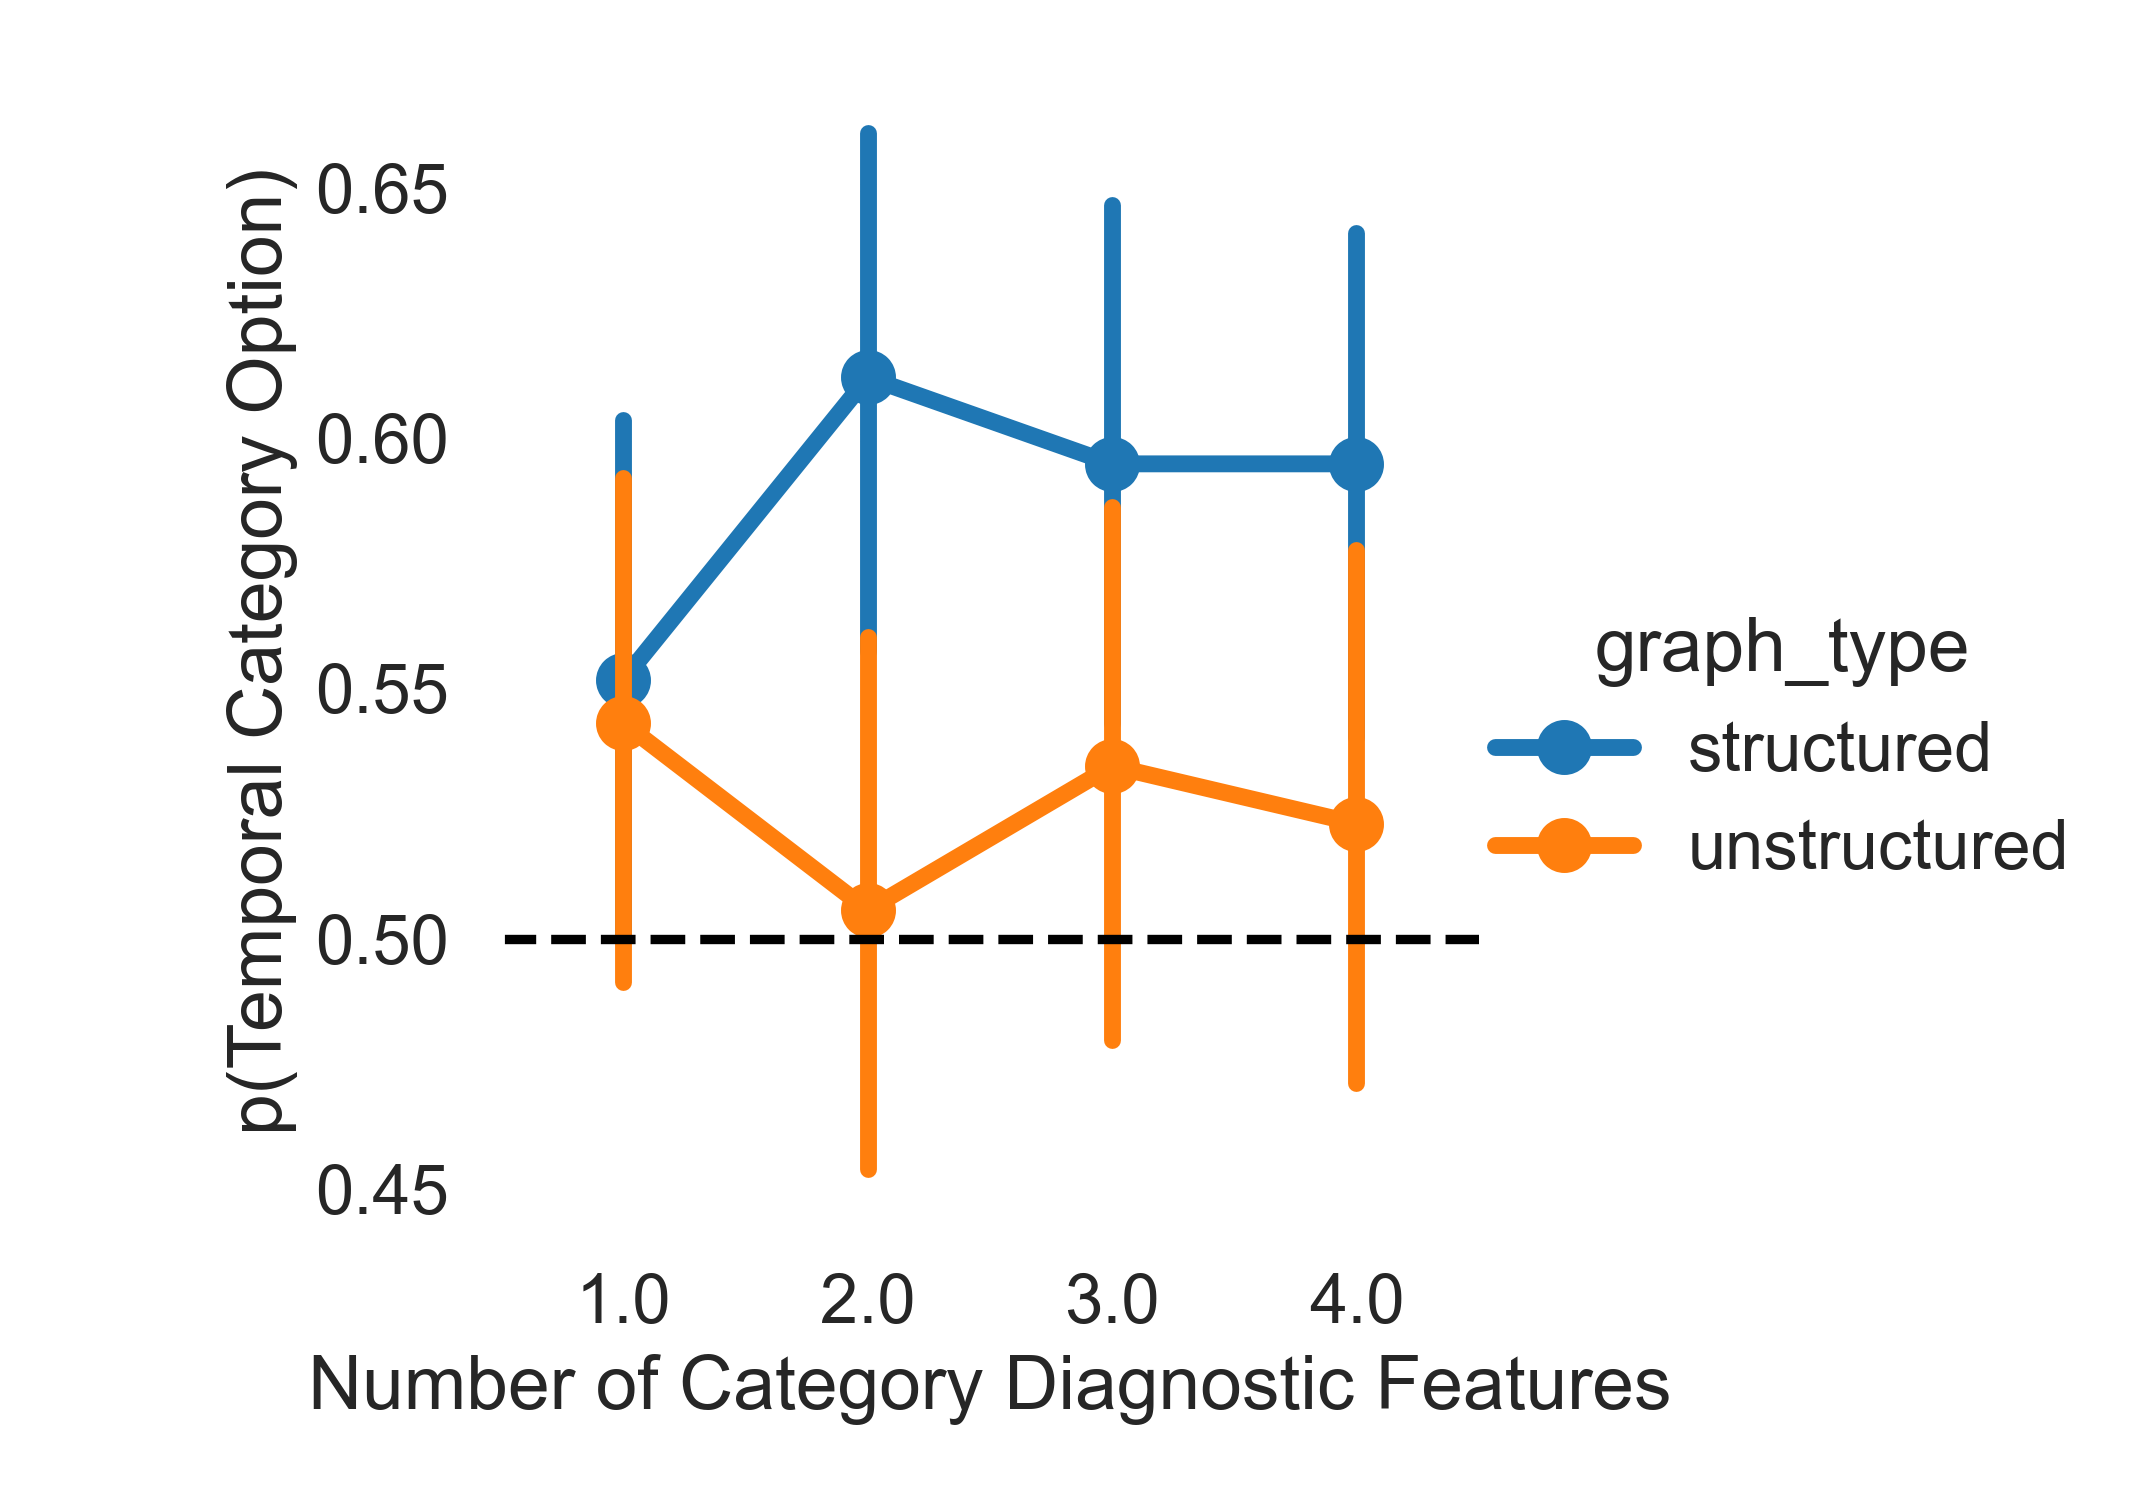
\includegraphics[width = \textwidth]{chapter_notebooks/chapter_4/figures/exp4_proportion_results.png}
    \label{fig:exp4a-choice-accuracy}
\end{figure}
The following bayesian model was used to estimate the effect sizes for categorization based on category diagnostic features for structured weighted walk relative to unstructured walk. 

\begin{equation}
    \begin{aligned}
        1|participant \sim \mathcal{N}(0, Half\mathcal{N}(3.65)) \\
        C(num\_feats):graph\_type \sim \mathcal{N}(0, 7.5) \\ 
        \mu = 0  + C(num\_feats):graph\_type + (1|participant) \\
        p(category\ diagnostic\ option) \sim Bernoulli(\mu) 
    \end{aligned}
\end{equation}

Posterior parameter distributions of chosing the option with common category diagnostic feature in the structured walk relative to unstructured walk are shown in figure \ref{fig:exp4a-bayesmodel-choice-accuracy}
\begin{figure}[h]
    \centering
    \caption{Bayesian estimates of proportions of temporally consistent features used as category diagnostic when exposed to structure relative to when not exposed to structure.}
    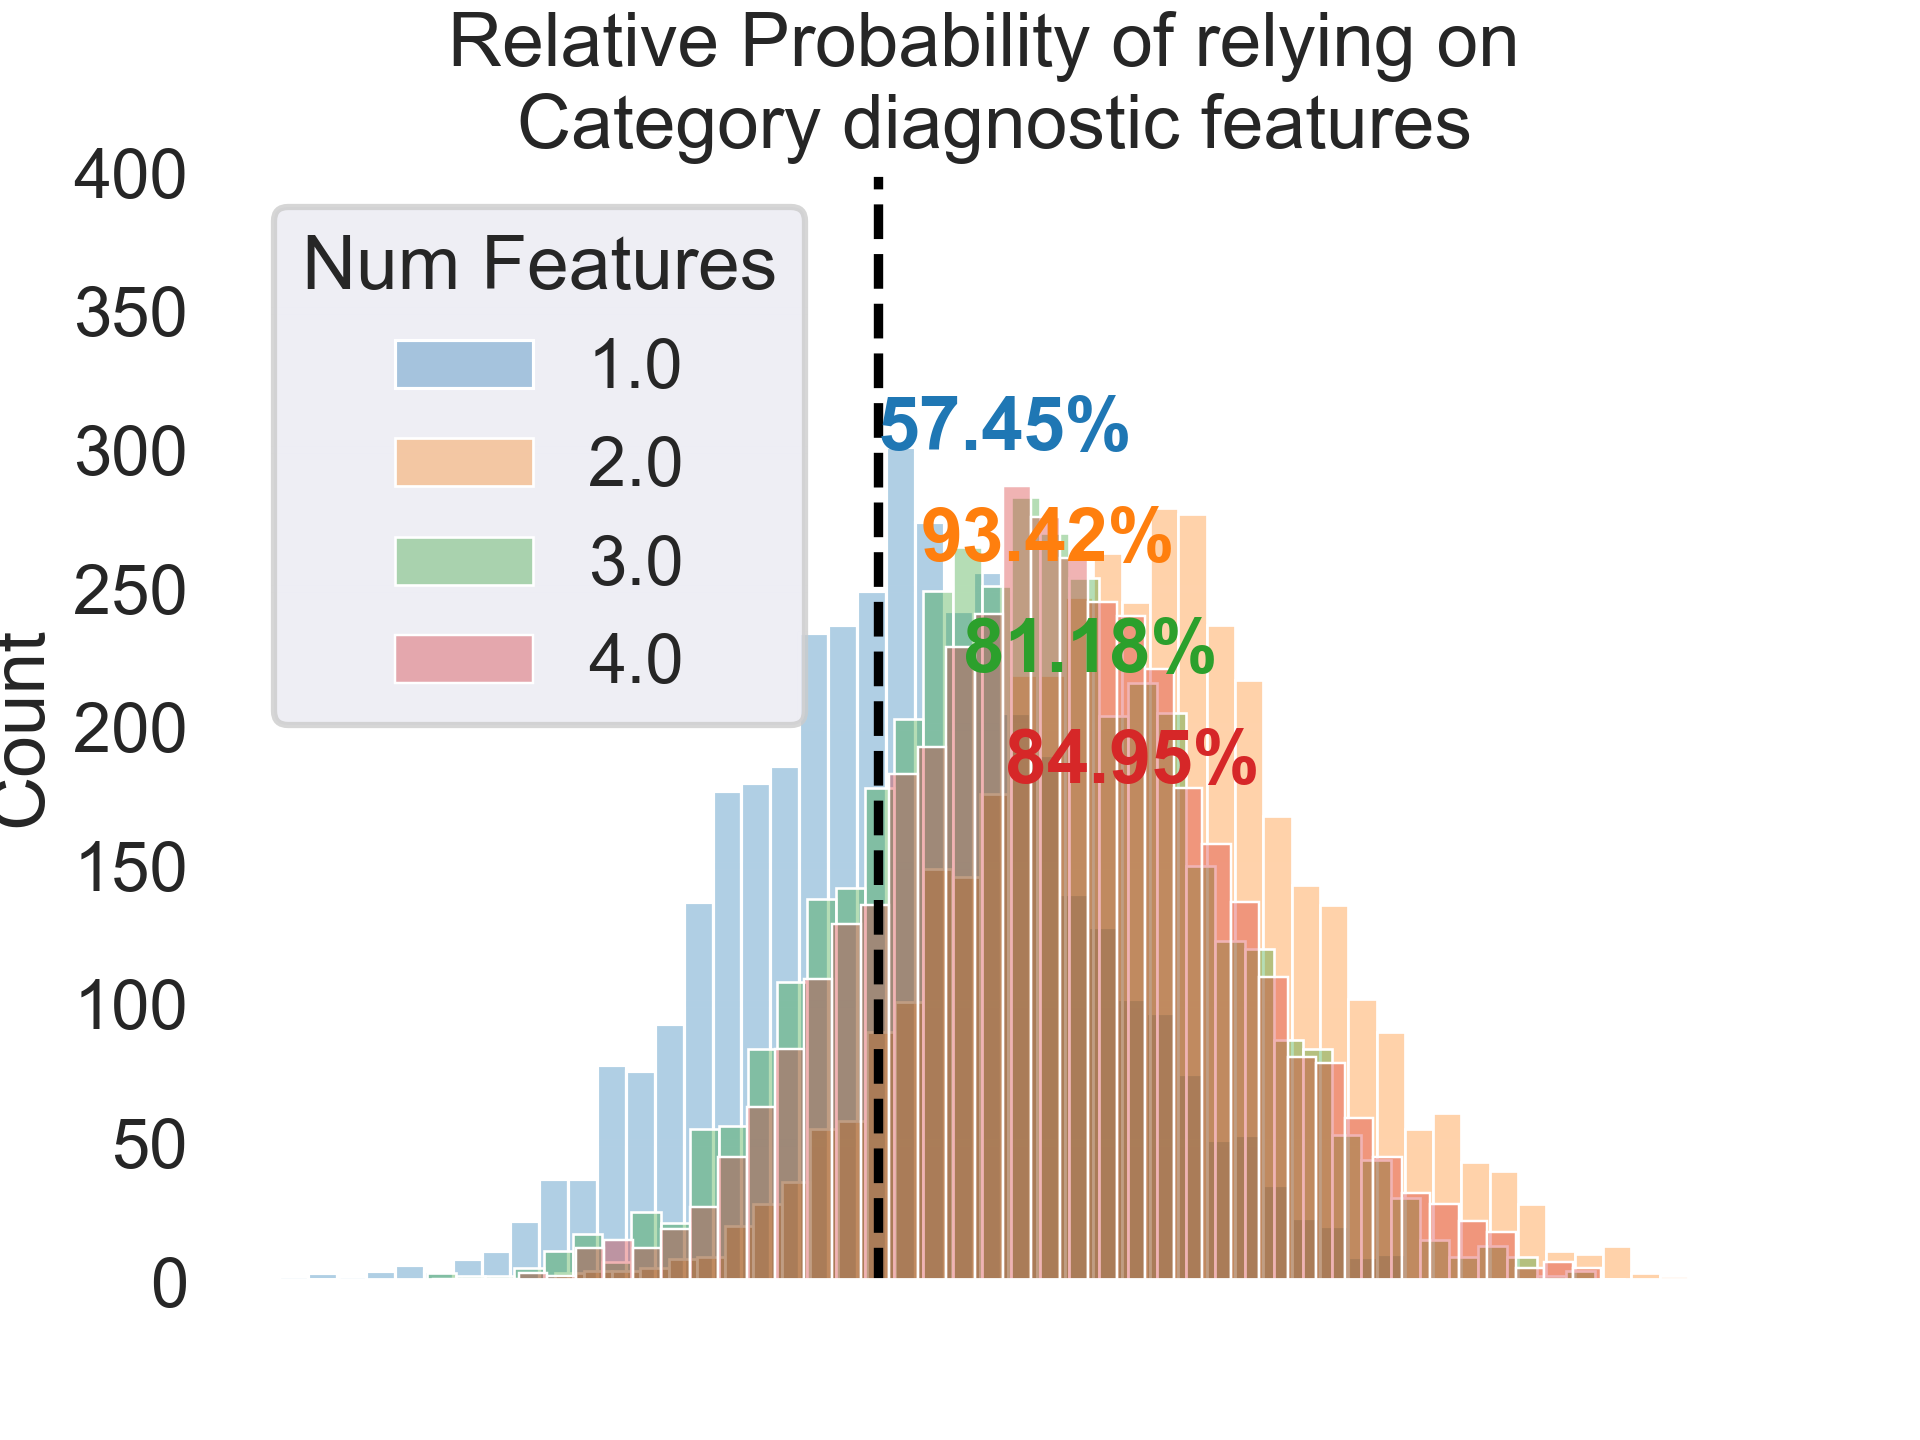
\includegraphics[width = \textwidth]{chapter_notebooks/chapter_4/figures/exp4_bayesmodel_res.png}
    \label{fig:exp4a-bayesmodel-choice-accuracy}
\end{figure}

Results from this experiment thus indicate that participants indeed pick up on features that are consistent between items that are temporally proximal. In the next experiment I aim to extend this finding to assess whether such temporal arrangements can be used as an \textit{intervention} to have participants learn arbitrary features as category diagnostic. Specifically, by using a limited set of features to define a category (as opposed to a pseudo-random selection in experiment 4a). Experiment 4b thus provides (1) An opportunity to replicate findings in experiment 4a, and (2) An assessment whether temporal proximity can be used as an experimental intervention to have participants learn category diagnostic features. 

\section{Experiment 3b}
\subsection{Methods}
\subsubsection*{Participants}
40 participants were recruited over Prolific to complete this 30-minute study. Participants were paid \$5 for their time. All study procedures were approved by the University of Massachusetts Institutional Review Board. 

\subsubsection*{Design and Procedure}
Two groups of participants experienced two different sets of features as category diagnostic. Both groups of participants experienced a weighted random walk during their exposure phase (similar to the structured condition in experiment 4a). For group A, one feature (out of two) for each of the four dimension was chosen to be category diagnostic. For group B, the other feature was category diagnostic. Specifically, head color, eye size, feet orientation, and nose shape were used as category diagnostic features for participants in group A. Torso color, arm length, antenna orientation, and bellybutton shape were used as category diagnostic features for participants in group B. All other experimental procedures were the same as in experiment 4a (see figure \ref{fig:exp45-deisgn}). 

\subsection{Results}
Figure \ref{fig:exp5-category-proportions} shows the proportion of categorization trials where a category diagnostic feature was used to classify the test item. 
\begin{figure}[h]
    \centering
    \caption{Proportion of categorization trials for which category diagnostic features were chosen to determine category membership}
    \label{fig:exp5-category-proportions}
    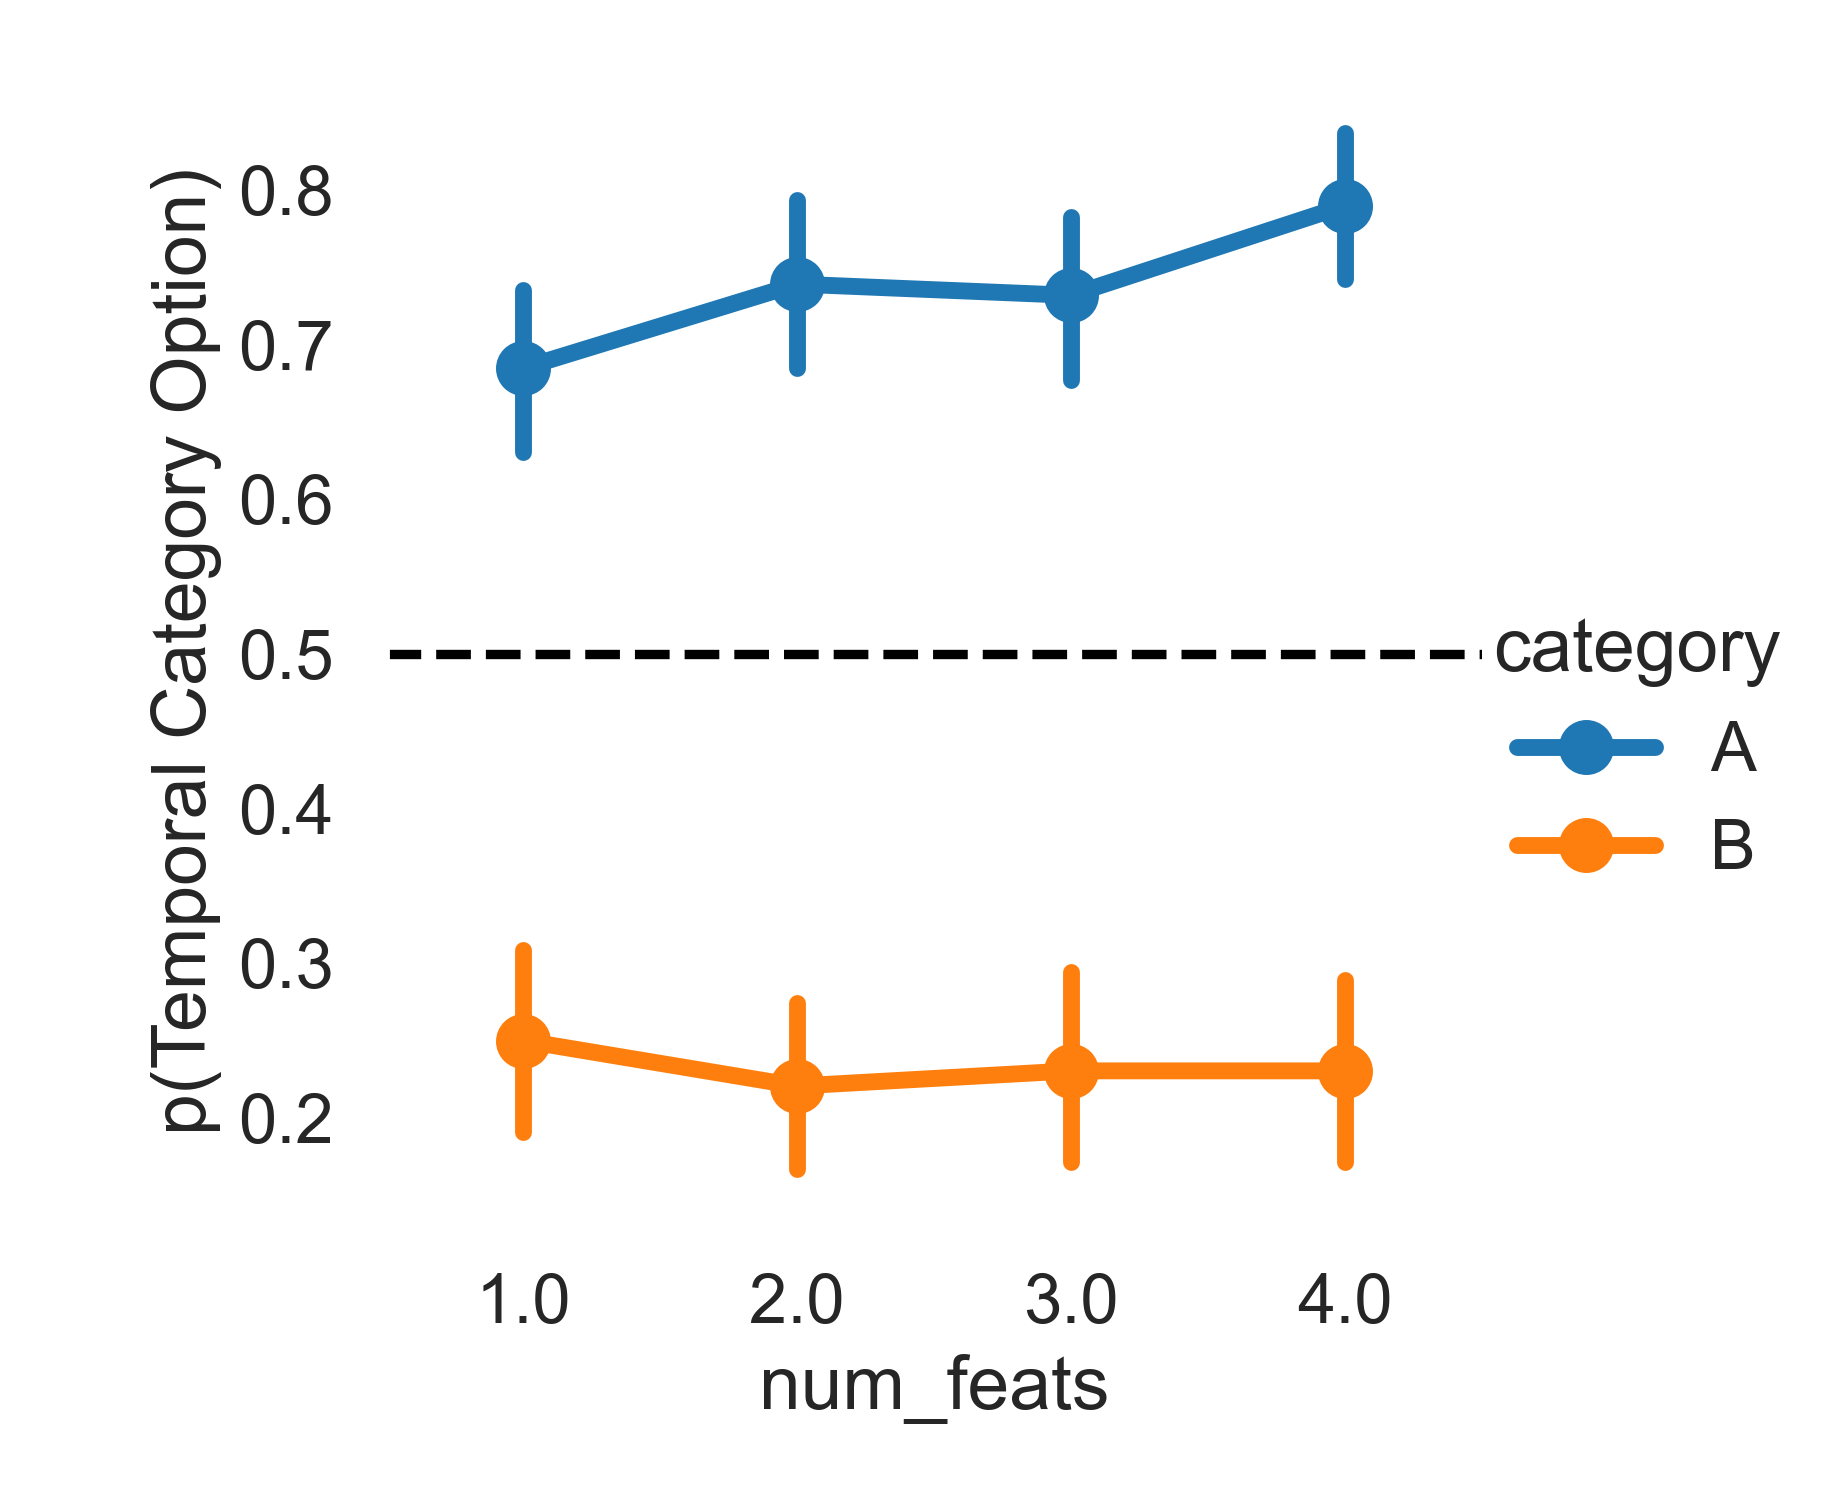
\includegraphics[width = \textwidth]{chapter_notebooks/chapter_4/figures/exp5_proportion_results.png}
\end{figure}
The same model as in experiment 4a was used to estimate effect sizes for both conditions. Figure \ref{fig:exp5-bayesian-estimates-proportions} shows the posterior estimates of these effect sizes. Interestingly, features that were category diagnostic for participants exposed to category A were used to categorize test items. On the other hand, features that were category diagnostic for participants exposed to category B were \textit{not} used; instead category non-diagnostic features (i.e. features that remained consistent during low probability transitions) were instead used to group the test item. 

\begin{figure}[h]
    \centering
    \caption{Bayesian posterior parameter estimates modeling the proportions of temporally consistent features used as category diagnostic for participants exposed to category A (\textit{left panel}) features as category diagnostic and when participants were exposed to category B features as category diagnostic. (\textit{Right panel})}
    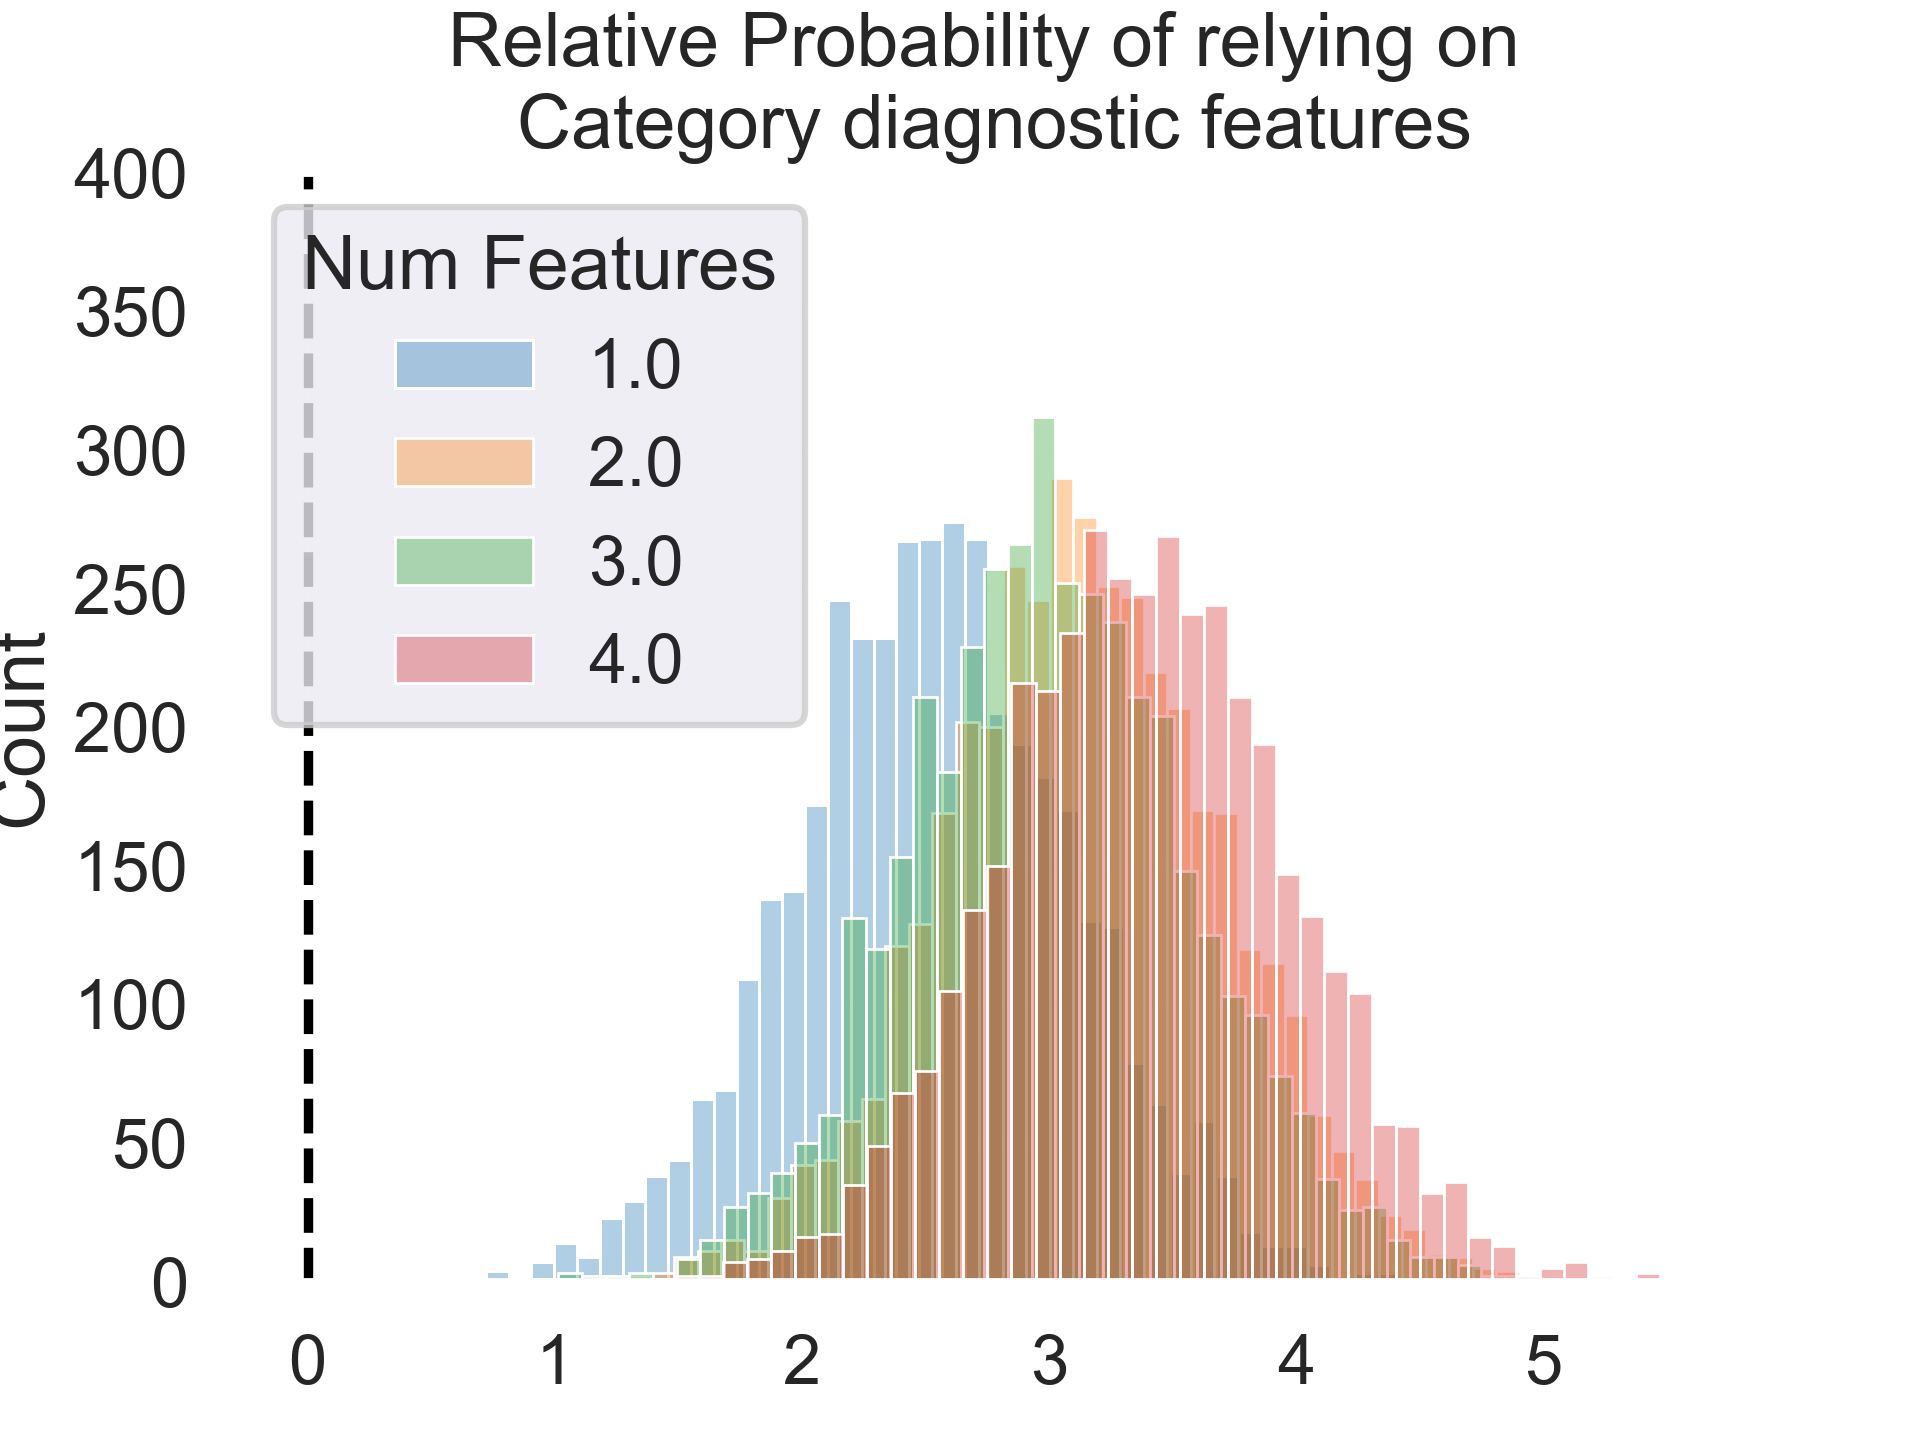
\includegraphics[width = \textwidth]{chapter_notebooks/chapter_4/figures/exp5_bayesmodel_res.png}
    \label{fig:exp5-bayesian-estimates-proportions}
\end{figure}



% In this article, we explore the effects of temporal co-occurrences to manipulate category membership. In particular, we follow the framework of the generalized context model (GCM) \cite{nosofsky1986attention,nosofsky1994comparing, rouder2004comparing}


\section{Discussion} 
The aim of this chapter was to assess if consistency of temporally proximal features leads to category formation. Experiments in this chapter follow a qualitatively similar design relative to past experiments assessing whether category formation is better with blocked design (where items from one category are presented serially after items from another category) compared to interleaved design (where items from all categories are presented together). Unlike past work, the present experiments investigate whether similar (or opposite) benefit exists for tasks where category formation is implicit -- until test, participants were not informed of any categorical structure in the stimuli. 

Past findings in explicit categorization have suggested that category formation is improved with interleaved presentation compared to blocked presentation. However, temporal proximity has been shown to increase representational similarity in the hippocampus \cite{schapiro2013neural}; blocked design may thus lead to realization of consistent patterns based on temporal proximity. Assuming SR as representation for temporal proximity, model simulations show that temporal proximity can indeed lead to categorization. 

Experiment 4a provides support for temporal proximity leading to categorization. However, experiment 4b leads to an interesting update to the model of category learning. When temporal proximity was used as an intervention to category learning, participants picked up on consistency of some features (category A) but on the \textit{differences} of the other features (category B) showing an interleave benefit. 

\subsection*{Model Update}
In the modeling approach shown earlier, two assumptions were made (1) All features were assumed to be equally weighted prior to exposure and (2) Feature weights were modified by consistency temporal proximity -- for each pair of stimuli, if they shared a feature, the weight of the shared feature was proportional to SR representation of the stimuli pairs.  

To incorporate results from experiment 4b, equation 4.2, can thus be modified as follows:

\begin{equation}
    \begin{aligned}
        w_m = w_b * \sum_{i, j}^{i_m == j_m} M(i, j)
    \end{aligned}
\end{equation}
where $w_b$ is the baseline weight for that feature. Updated model simulations are in figure \ref{fig:category-sr-sims-updated}

\begin{figure}
    \centering
    \label{fig:category-sr-sims-updated}
    \caption{Updated model simulations. Base feature weights determine whether more weight is placed on proximally similar \textit{(right panel)} or proximally distinct features \textit{(left panel)}.}
    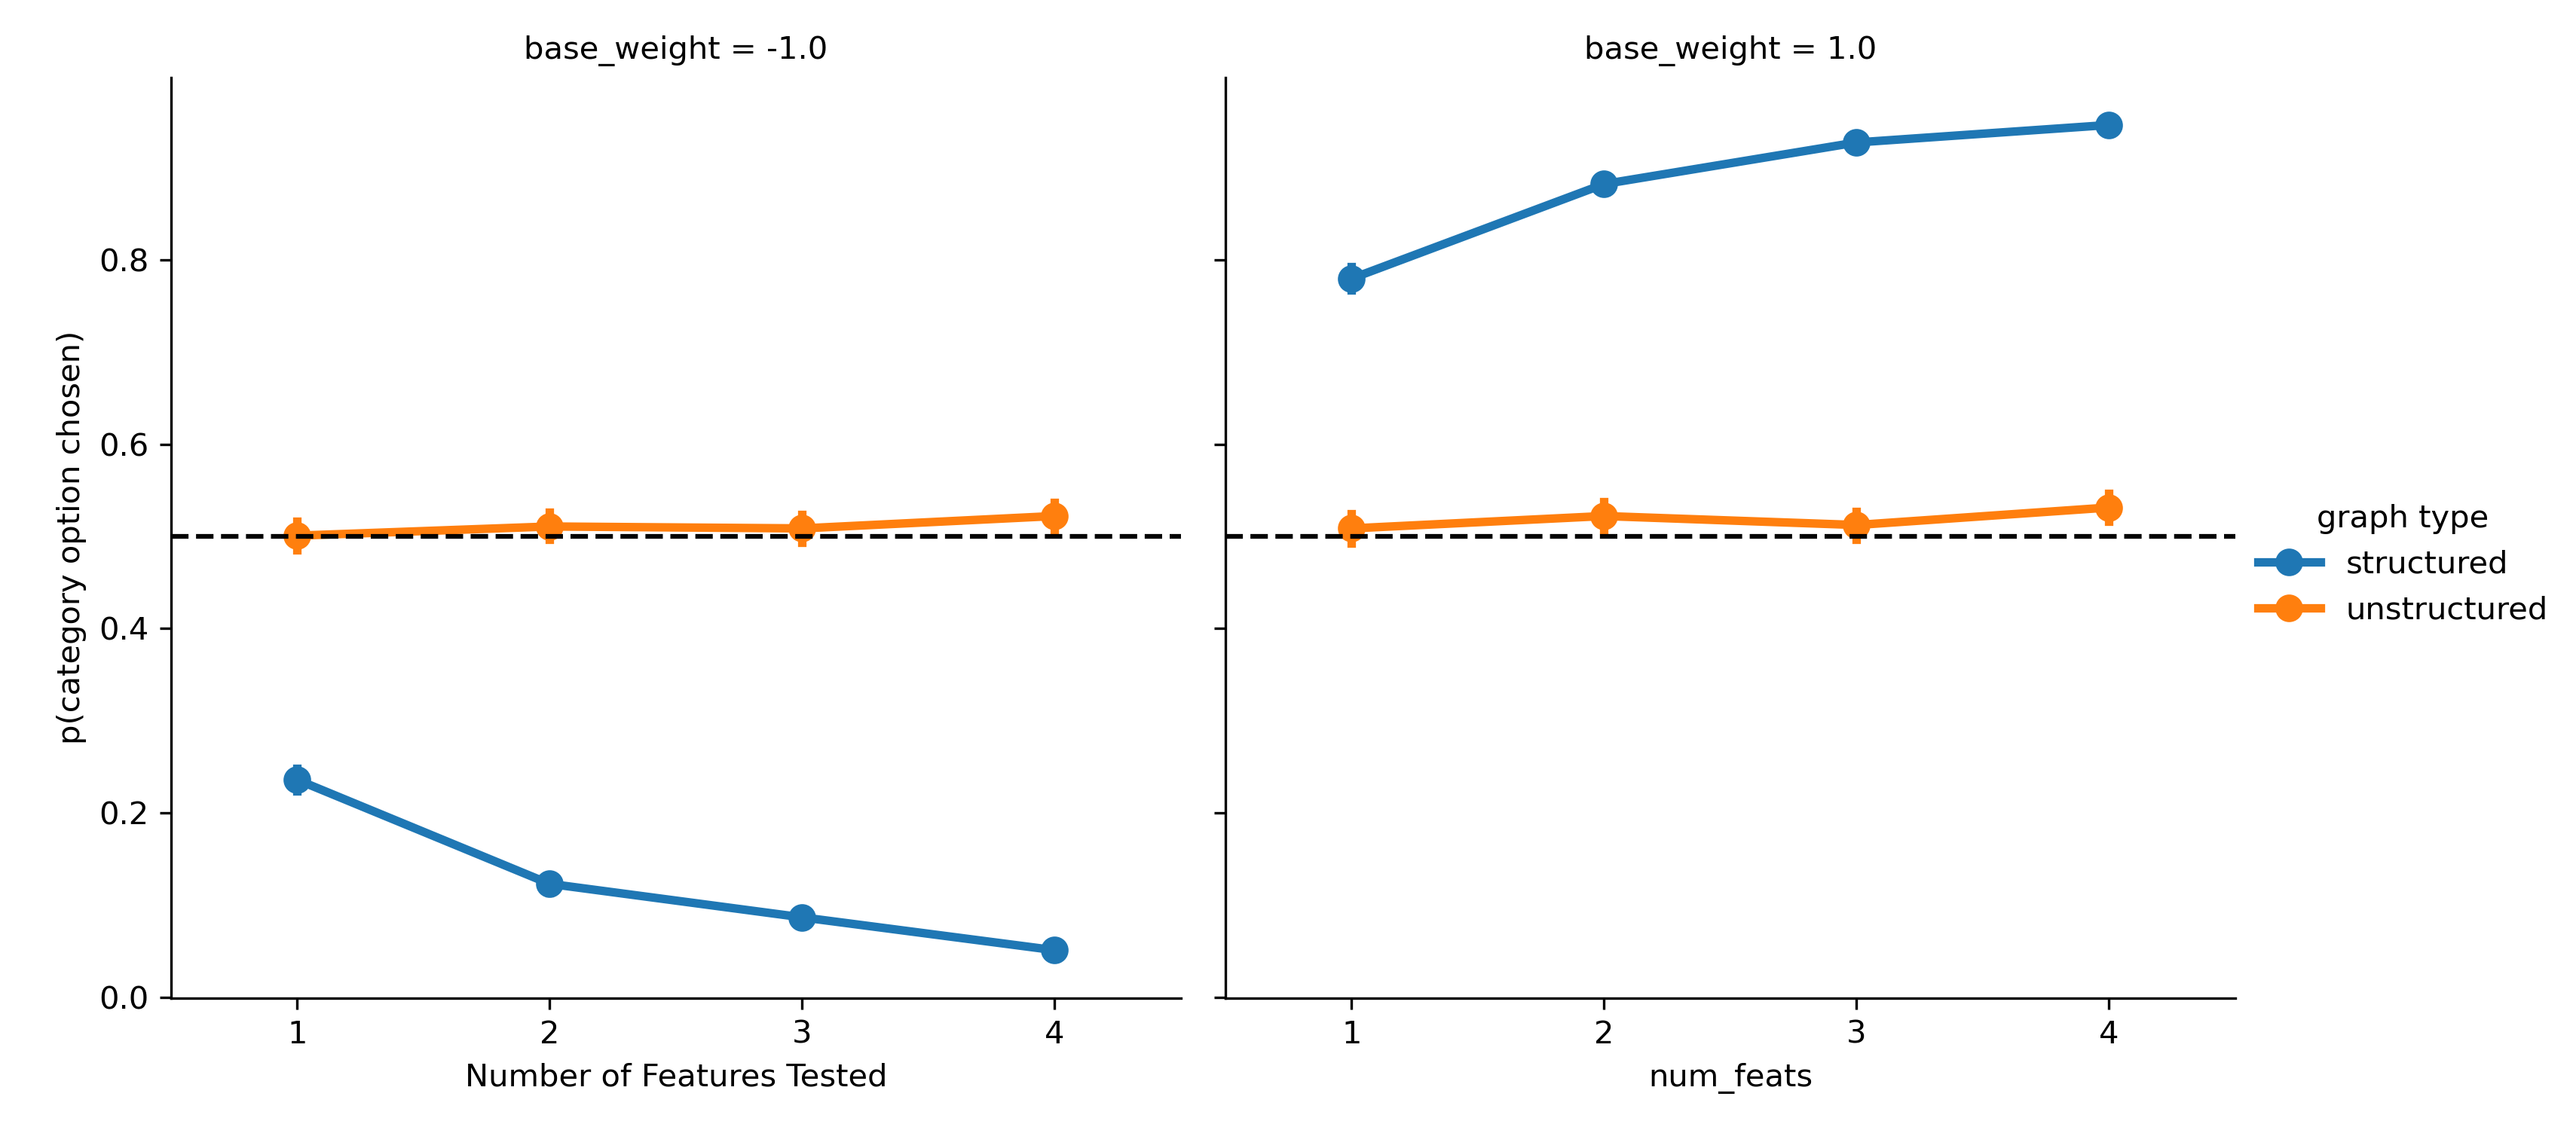
\includegraphics[width = \textwidth]{chapter_notebooks/chapter_4/figures/cat_simulations_baseweights.png}
\end{figure}

The updated model allows for interleaving benefit by increasing the proximally non-consistent feature weights. It is unclear what features lead to an increased attention weight on differences (as would be the case for interleaved categories) or an increased attention weight on consistencies (for blocked categories). Perhaps, features that are more notable lead to an interleaving benefit as more frequent changes in feature values of more notable features become apparent. Norming studies in future experiments can address whether temporal attention benefit depends on baseline noticeability. 

\section{Conclusion}
In this chapter, I demonstrate a use of a context representation framework (specifically predictive representation using SR) to understand the mechanisms behind implicit category learning based on temporal relationships. Findings of these experiments can further model considerations in classical categorization models such as the GCM to incorporate information about temporal presentation order in assigning feature weights. More broadly, given that temporal associations seem to have an effect on how things are visually categorized (albeit, dependent on the specific feature), manipulating temporal associations can be used in more practical settings such as learning natural categories in classrooms. (For example when training students to visually recognize types of geological rocks \cite{nosofsky2018toward, nosofsky2017learning}). 